\chapter{The Geometry of Vector Spaces}
In this chapter we do stuff.
\section{The Geometry of $\mathbb{R}^n$}
At this point we have talked almost exclusively about linear combinations and the spaces
associated with them.  We have not, however, discussed the geometry of vector spaces.  So
far we haven't generalized the notions of angle and length of vectors to our large view of
vector spaces.  You may recall things like projections, angles, norms (lengths) from
$\mathbb{R}^2$ or $\mathbb{R}^3$ as discussed in physics or in multivariable calculus but
you need to keep in mind that this is only a limited view of the world of vector spaces.
Let's jump right in by filling in some definitions and theorems that you likely already
know

\subsection{The Dot Product}
Now let's summarize our results in the following definitions and theorems.
\begin{definition}[Dot Product in $\mathbb{R}^n$]
    Let $\bu, \bv \in \mathbb{R}^n$.  The {\bf dot product} of $\bu$ and $\bv$ is defined
    algebraically as
    \[ \bu \cdot \bv = \underline{\hspace{2in}} \]
    (this definition doesn't explicitly mention the angle between the vectors)
\end{definition}
\solution{
    $\bu \cdot \bv = \sum_{j=1}^n u_j v_j$
}

\begin{definition}[Dot Product and Vector Angles]
    If $\bu,\bv\in\mathbb{R}^n$ then the relationship between the dot product of the
    vectors and the angle between the vectors is
    \[ \bu \cdot \bv = \underline{\hspace{2in}} \]
\end{definition}
\solution{
$\bu \cdot \bv = \|\bu\| \|\bv\| \cos \theta$
}

\begin{thm}[Orthogonal Vectors in $\mathbb{R}^n$]
    If $\bu,\bv\in\mathbb{R}^n$ then $\bu$ is orthogonal (perpendicular) to $\bv$ if and
    only if \underline{\hspace{1in}}.
\end{thm}
\solution{
$\bu \cdot \bv = 0$
}
\begin{proof}
    (prove this theorem)
\end{proof}
\solution{
$\bu \cdot \bv = \|\bv \| \|\bu\| \cos \theta$ and since $\theta = \pi/2$ we know that
$\cos \theta = 0$.  Hence $\bu \cdot \bv = 0$.
}

\begin{definition}[Length of Vectors in $\mathbb{R}^n$]
    Let $\bu \in \mathbb{R}^n$.  The {\bf length (norm)} of $\bu$ is
    \[ \| \bu \| = \sqrt{\bu \cdot \bu} = \underline{\hspace{2in}} \]
\end{definition}
\solution{
    $\|\bu\| = \sum_{j=1}^n u_j^2$
}

\begin{definition}[Distance Between Vectors in $\mathbb{R}^n$]
    Let $\bu,\bv\in\mathbb{R}^n$.  The {\bf distance between} $\bu$ and $\bv$ is
    \[ \text{dist}(\bu,\bv) = \underline{\hspace{1in}} \]
\end{definition}
\solution{
    $\text{dist}(\bu,\bv) = \|\bu-\bv\|$
}


\subsection{Projections}
Finally we are going to discuss projections.  When dealing with projections you should be
thinking about how shadows are cast between vectors.  To solidify this notion (even though
you likely already know it) let's look at some projections in $\mathbb{R}^2$ before we
ramp up the dimension.  Take a look at Figure \ref{fig:proj_R2}.  We would like to project
vector $\bu$ onto vector $\bv$ and by that we mean that we would like to draw a vector
(depicted by the dashed vector $\bw$ in the figure) that is perpendicular to $\bv$ and meets the
head of $\bu$. This projection creates the vector $\hat{\bv}$ so that $\hat{\bv}$ points
in exactly the same direction as $\bv$ but $\hat{\bv} \perp \bw$. Since $\bv$ and
$\hat{\bv}$ point in the same direction we know that $\hat{\bv} = c\bv$ for some scalar
$c$.  Furthermore, we know that $\bw + \hat{\bv} = \bu$ so $\bw = \bu - \hat{\bv}$. Therefore,
\begin{flalign*}
    &0 = \hat{\bv} \cdot \bw = c\bv \cdot \left( \bu - c\bv \right) \\
    &\implies c\bv \cdot \bu - c^2 \bv \cdot \bv = 0 \\
    &\implies \bu \cdot \bv = c \bv \cdot \bv \\
    &\implies c = \frac{\bu \cdot \bv}{\bv \cdot \bv}
\end{flalign*}
\begin{figure}[ht!]
    \begin{center}
        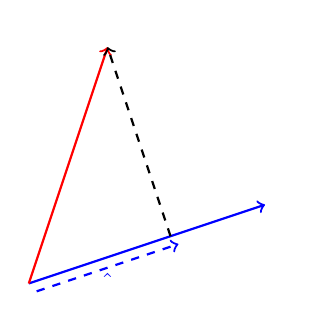
\begin{tikzpicture}
            \draw[->,thick, blue] (0,0) -- (3,1) node[anchor=west]{$\bv$};
            \draw[->,thick, red] (0,0) -- (1,3) node[anchor=south]{$\bu$};
            \draw[->,thick, dashed, black] (1.8,0.6) -- (1,3);
            \draw[black] (1.4,2) node[anchor=west]{$\bw$};
            \draw[->,thick, dashed, blue] (0.1,-0.1) -- (1.9,0.5);
            \draw[blue] (1,0.25) node[anchor=north]{$\hat{\bv}$};
        \end{tikzpicture}
    \end{center}
    \caption{Depiction of vector projection in $\mathbb{R}^2$.}
    \label{fig:proj_R2}
\end{figure}

All of the prior discuss proves the following theorem but notice that we never made any
mention explicitly about the vectors living in $\mathbb{R}^2$.  In fact, the proof that we
gave works generally in $\mathbb{R}^n$.
\begin{thm}[Orthogonal Projection]
    Let $\bu, \bv \in \mathbb{R}^n$.  If we are to project $\bu$ onto $\bv$ as in Figure
    \ref{fig:proj_R2} we get
    \begin{flalign*}
        \text{proj}_{\bv}(\bu) &= \hat{\bv} = \left( \frac{\bv \cdot \bu}{\bv \cdot \bv}
        \right) \bv =
        \text{projection of $\bu$ onto $\bv$} \\
        \bw &= \bu - \hat{\bv} = \bu - \left( \frac{\bv \cdot \bu}{\bv \cdot \bv} \right)
        \bv
        = \text{projection error}
    \end{flalign*}
    The vector $\bw$ is often called the {\it error} in the projection.
\end{thm}




\begin{problem}
    What is the dot product of 
    $\left( \begin{array}{c} 0 \\ 1 \\ -1 \end{array} \right)$ and 
    $\left( \begin{array}{c} 4 \\ 2 \\ -3 \end{array} \right)$?

\begin{enumerate}
    \item[(a)] 
$\left( \begin{array}{c} 0 \\ 2 \\ 3 \end{array} \right)$
\item[(b)] 5
\item[(c)] 0
\item[(d)] The dot product cannot be computed for these vectors.
\end{enumerate}
\end{problem}
% \begin{problem}
%     \begin{itemize}
%             \input{ClickerQuestions/LA.00.22.010}
%     \end{itemize}
% \end{problem}
\solution{
$(0)(4) + (1)(2) + (-1)(-3) = 2+3 = 5$
}


\begin{problem}
    If $\bb = \left( \begin{array}{c} 3 \\ -1  \end{array} \right)$ and $y = \left(
    \begin{array}{c} 2 \\ 1  \end{array} \right),$ then the orthogonal projection of $\bb$
    onto $\by$ is

\begin{enumerate}
    \item[(a)] $\left( \begin{array}{c} 2 \\ 1  \end{array} \right)$
    \item[(b)] $\left( \begin{array}{c} 3/2 \\ -1/2 \end{array} \right)$
    \item[(c)] $\left( \begin{array}{c} 10 \\ 5  \end{array} \right)$
    \item[(d)] $\left( \begin{array}{c} 1/10 \\ 3/10  \end{array} \right)$
\end{enumerate}

\end{problem}
% \begin{problem}
%     \begin{itemize}
%             \input{ClickerQuestions/LA.00.24.010}
%     \end{itemize}
% \end{problem}
\solution{
    $\text{proj}_y b = \left( \frac{b \cdot y}{y \dot y} \right) y = \left(
    \frac{5}{5}
    \right) \begin{pmatrix} 2 \\ 1 \end{pmatrix} = \begin{pmatrix}2\\1\end{pmatrix}$
}


\begin{problem}
    If $\mathcal{B} = \{\bv_1, \bv_2, \ldots, \bv_n\}$ is an orthogonal basis for a vector
    space $\mathcal{V}$ then how do you write $\bx$ as a linear combination of the basis vectors?\\
    (Why is it advantageous to have an orthogonal basis?) 
    Hint: Since $\bx = c_1 \bv_1 + c_2 \bv_2 + \cdots + c_n \bv_n$ how can you use
    orthogonality to solve for $c_j$?
\end{problem}
\solution{
    $c_j = \frac{\bx \cdot \bv_j}{\bv_j \cdot \bv_j}$
}

\begin{problem}
    Implement your idea on the subspace spanned by the basis
    \[ \mathcal{B} = \left\{ \begin{pmatrix} 1\\4\\-3 \end{pmatrix}\, , \, \begin{pmatrix}
            3 \\ 0 \\ 1 \end{pmatrix} \right\} \]
    where $\bx$ is in the subspace of $\mathbb{R}^3$ spanned by $\mathcal{B}$
    \[ \bx = \begin{pmatrix} 2 \\ -4\\ 1 \end{pmatrix} \]
\end{problem}
\solution{
    Since $\bx = c_1 \begin{pmatrix} 1 \\ 4 \\ -3 \end{pmatrix} + c_2 \begin{pmatrix} 3 \\ 0 \\
        1 \end{pmatrix}$ so 
    \[ c_1 = \frac{\bx \cdot \bv_1}{\bv_1 \cdot \bv_1} = \frac{-17}{26} \]
    \[ c_2 = \frac{\bx \cdot \bv_2}{\bv_2 \cdot \bv_2} = \frac{7}{10} \]
}

Now summarize the process that you built in the previous problem into the following
theorem.
\begin{thm}[Building Vectors from an Orthogonal Basis]\label{thm:orthogonal_basis}
    If $\mathcal{B} = \{\bv_1, \bv_2, \ldots, \bv_n\}$ is an orthogonal basis for a vector
    space $\mathcal{V}$ then for $\bx \in \mathcal{V}$
    \[ \bx = \underline{\hspace{0.25in}} \bv_1 + \underline{\hspace{0.25in}} \bv_2 +
    \underline{\hspace{0.25in}} \bv_3 + \cdots + \underline{\hspace{0.25in}} \bv_n \]
    (Fill in the blanks)
\end{thm}
\solution{
    $c_j = \frac{\bx \cdot \bv_j}{\bv_j \cdot \bv_j}$
}


\begin{thm}
    If the nonzero vectors $\bu_1, \bu_2, \bu_2, \dots, \bu_k$ are mutually orthogonal
    then they are linearly independent.
\end{thm}
\begin{proof}
    (prove this theorem)
\end{proof}
\solution{
    Consider $\bo = \sum_{j=1}^n c_j \bu_j$.  From the previous theorem we know that $c_j
    = (\bo \cdot \bu_j) / (\bu_j \cdot \bu_j) = 0$.  Therefore the only solution is the
    trivial solution and the vectors must be linearly independent.
}


\begin{problem}
    Determine if the following set of vectors is linearly independent.  Do this two
    different ways.
    \[ \left\{ \begin{pmatrix} 3 \\ 1 \\ 1 \end{pmatrix} \, , \, \begin{pmatrix} -1 \\ 2
            \\ 1
    \end{pmatrix} \, , \, \begin{pmatrix} -1 \\ -4 \\ 7 \end{pmatrix} \right\} \]
\end{problem}
\solution{
They are mutually orthogonal so they are linearly independent.
}







\begin{problem}
    If we have two linearly independent vectors that are NOT orthogonal, how do
    we find a set of two orthogonal vectors that span the same space?

    For example, can we find two orthogonal vectors that span the same space as
    \[ \begin{pmatrix} 2 \\ 0 \end{pmatrix} \quad \text{and} \quad \begin{pmatrix} 1
        \\ 1 \end{pmatrix} \]
\end{problem}

\subsection{The Gram-Schmidt Process: Making Orthogonal Sets}
The previous theorems and problems give us good reason to think that having an orthogonal
(or orthonormal) basis for a vector space is advantageous both computationally and
geometrically.  In fact, we have been used to an orthonormal basis all of our matheamtical
lives since that is what the regular Cartesian coordinate system is built from.  The
question now is this: \\
Given a basis $\mathcal{B}$ for a vector space $\mathcal{V}$ how can we transform that
basis into a different basis for the same space but also gain orthogonality?
We will build your intuition to the process via a scaffolded problem.  

\begin{problem}
    Build a basis for $\mathbb{R}^2$ so that it contains two orthogonal unit vectors with
    one of the vectors parallel to $\bv_1 = \begin{pmatrix} 1\\1\end{pmatrix}$.
\end{problem}

\begin{problem}
    Consider the vector space $\mathbb{R}^3$ with the basis $\mathcal{B} = \{\bv_1, \bv_2,
    \bv_3\}$ given by
    \[ \bv_1 = \begin{pmatrix} 1\\1\\1\end{pmatrix}, \quad \bv_2 = \begin{pmatrix} 0
            \\1\\1\end{pmatrix},\quad \bv_3 = \begin{pmatrix} 0\\0\\1\end{pmatrix} \]
                We are going to build a basis $\mathcal{U} = \{\bu_1, \bu_2, \bu_3\}$ such that $\text{span}(\mathcal{U}) =
    \mathbb{R}^3$ but the vectors are also mutually orthogonal and all have unit length.
    (One should note here that the normalization step is optional but since unit vectors
    are so nice to work with we are leaving it here.)
    \begin{enumerate}
        \item[(a)] Define $\bu_1$ as a unit vector that points in the same direction as
            $\bv_1$.
            \[ \bu_1 = \frac{1}{\|\bv_1\|} \bv_1 =  \begin{pmatrix} \underline{\hspace{0.25in}} \\
                    \underline{\hspace{0.25in}} \\ \underline{\hspace{0.25in}} \end{pmatrix}
                    \]
\solution{
    $\bu_1 = \frac{1}{\sqrt{3}} \begin{pmatrix} 1\\1\\1\end{pmatrix} = \begin{pmatrix}
        1/\sqrt{3} \\ 1/\sqrt{3} \\ 1/\sqrt{3} \end{pmatrix}$
}
        \item[(b)] Now we project $\bv_2$ onto $\bu_1$ and find the error in the
            projection.  This would be the vector $\bw$ in Figure \ref{fig:proj_R2}.  Once
            we have the error we should normalize it to get $\bu_2$.
            \[ \bw_2 = \bv_2 - \text{proj}_{\bu}(\bv_2) = \bv_2 - \left( \bv_2 \cdot \bu_1
                \right) \bu_1 \quad \text{and therefore} \quad \bu_2 =
                \frac{1}{\|\bw_2\|}\bw_2. \]
            Draw a picture of what we just did.
            \[ \bu_2 = \frac{1}{\|\bv_1\|} \bv_1 =  \begin{pmatrix}
                    \underline{\hspace{0.25in}} \\ \underline{\hspace{0.25in}} \\
                    \underline{\hspace{0.25in}} \end{pmatrix} \]
\solution{
    $\bw_2 = \begin{pmatrix} 0\\1\\1\end{pmatrix} - \left( \frac{2}{\sqrt{3}}
        \right)\begin{pmatrix} 1/\sqrt{3} \\ 1/\sqrt{3} \\ 1/\sqrt{3} \end{pmatrix} =
            \begin{pmatrix}0\\1\\1\end{pmatrix} - \begin{pmatrix} 2/3 \\ 2/3 \\ 2/3
            \end{pmatrix} = \begin{pmatrix} -2/3 \\ 1/3 \\ 1/3 \end{pmatrix}$.  Therefore
                $\bu_2 = \frac{1}{\|\bw_2\|}\bw_2 $ so
                \[ \bu_2 = \frac{\sqrt{3}}{\sqrt{2}} \begin{pmatrix} -2/3 \\ 1/3 \\
                        1/3\end{pmatrix} = \frac{1}{\sqrt{6}} \begin{pmatrix}
                            -2\\1\\1\end{pmatrix} = \begin{pmatrix} -2/\sqrt{6} \\
                                1/\sqrt{6} \\ 1/\sqrt{6} \end{pmatrix} \]
}
        \item[(c)] For $\bu_3$ we project $\bv_3$ onto both $\bu_1$ and $\bu_2$ and then
            normalize.
            \[ \bw_3 = \bv_3 - \left( \bv_3 \cdot \bu_1 \right)\bu_1 - \left( \bv_3 \cdot
                \bu_2
                \right) \bu_2 \quad \text{and therefore} \quad \bu_3 =
                \frac{1}{\|\bw_3\|}\bw_3 \]
            \[ \bu_3 = \frac{1}{\|\bv_1\|} \bv_1 =  \begin{pmatrix}
                    \underline{\hspace{0.25in}} \\ \underline{\hspace{0.25in}} \\
                    \underline{\hspace{0.25in}} \end{pmatrix} \]
\solution{
    \[ \bw_3 = \bv_3 - \left( \frac{1}{\sqrt{3}} \right)\begin{pmatrix} 1/\sqrt{3} \\
            1/\sqrt{3} \\ 1/\sqrt{3} \end{pmatrix} - \left( \frac{1}{\sqrt{6}} \right)
            \begin{pmatrix} -2/\sqrt{6} \\ 1/\sqrt{6} \\ 1/\sqrt{6} \end{pmatrix} =
                \begin{pmatrix}0\\0\\1\end{pmatrix} - \begin{pmatrix}1/3 \\ 1/3 \\ 1/3
                \end{pmatrix} - \begin{pmatrix} -2/6 \\ 1/6 \\ 1/6 \end{pmatrix} =
                    \begin{pmatrix} 0 \\ -1/2 \\ 1/2 \end{pmatrix} =
                        \frac{1}{2} \begin{pmatrix}0\\-1\\1\end{pmatrix} \]
    Therefore, we can build $\bu_3$ by normalizing
    \[ \bu_3 = \frac{\sqrt{2}}{2} \begin{pmatrix} 0\\-1\\1 \end{pmatrix}  =
            \frac{1}{\sqrt{2}} \begin{pmatrix} 0\\-1\\1\end{pmatrix} = \begin{pmatrix}
                0\\-1/\sqrt{2} \\ 1/\sqrt{2} \end{pmatrix}\]
}
        \item[(d)] Verify that indeed $\mathcal{U} = \{\bu_1, \bu_2, \bu_3\}$ is an
            orthonormal basis for $\mathbb{R}^3$.
\solution{
The orthonormal basis is:
\[ \mathcal{U} = \left\{ \begin{pmatrix} 1/\sqrt{3} \\ 1/\sqrt{3} \\ 1/\sqrt{3}
    \end{pmatrix} \, , \, \begin{pmatrix} -2/\sqrt{6} \\ 1/\sqrt{6} \\ 1/\sqrt{6}
    \end{pmatrix} \, , \, \begin{pmatrix} 0 \\ -1/\sqrt{2} \\ 1/\sqrt{2} \end{pmatrix}
    \right\} \]
    and we leave it to the reader to verify that indeed the vectors are mutually
    orthogonal.
}
    \end{enumerate}
\end{problem}


\begin{problem}
    Use the Gram-Schmidt process outlined in the previous problem to produce an orthogonal
    basis $\mathcal{U}$ for the subspace spanned by
    \[ \begin{pmatrix} 3\\0\\-1\end{pmatrix} \quad \text{and} \quad \begin{pmatrix}
            8\\5\\-6\end{pmatrix}. \]
\end{problem}

\begin{problem}
    Let's build an orthogonal basis $\mathcal{U}$ for $\mathbb{R}^3$.  To get started let
    $\bu_1 = \begin{pmatrix} 1\\0\\1\end{pmatrix}$.  (notice that we are not
        normalizing this time)
        \begin{enumerate}
            \item[(a)] Create a vector $\bu_2$ in $\mathbb{R}^3$ so that $\bu_1 \perp
                \bu_2$.
\solution{
A simple choice is $\bu_2 = (0,1,0)^T$.
}
            \item[(b)] Pick a vector $\bv_3 \in \mathbb{R}^3$ such that $\bv_3$ is
                linearly independent of $\bu_1$ and $\bu_2$.  Then use one step of the
                Gram-Schmidt process to create $\bu_3$ out of $\bv_3$.
\solution{One choice is $\bv_3 = (2,0,1)^T$.  Therefore
    \[ \bu_3 = \bv_3 - \left( \frac{\bv_3 \cdot \bu_1}{\|\bu_1\|^2} \right)\bu_1 - \left(
        \frac{\bv_3 \cdot \bu_2}{\|\bu_2\|^2}\right) \bu_2 = \begin{pmatrix}
            2\\0\\1\end{pmatrix} - \frac{3}{2}\begin{pmatrix} 1\\0\\1\end{pmatrix} - 0
                \begin{pmatrix} 0\\1\\0\end{pmatrix} = \begin{pmatrix} 1/2 \\ 0 \\
                    -1/2\end{pmatrix} \]
}
            \item[(c)] Verify that the vectors in your proposed basis are indeed mutually
                orthogonal.  If so we can use one of the previous theorems (which one) to
                say that the vectors are linearly independent and must therefore span
                $\mathbb{R}^3$.
\solution{It is trivial to verify that the three vectors are indeed mutually orthogonal.
}
        \end{enumerate}
\end{problem}


\section{Inner Product Spaces}
Now time for some more abstraction!  In this section we take the notions of geometry and
abstract them to generalized vector spaces.  You may have noticed that the dot product is
the basic computation necessary to understand angle in $\mathbb{R}^n$ so we first have to
provide a generalized version of the dot product.

\begin{definition}[The Inner Product]
    An {\bf inner product} is the abstraction of a dot product to a general vector space.
    If $\bu$, $\bv$, and $\bw$ are vectors in a vector space $\mathcal{V}$ and $c$ is some real
    number then
        \begin{enumerate}
            \item $\left< \bu,\bv\right> = \left<\bv,\bu\right>$
            \item $\left< \bu,\bv + \bw\right> = \left< \bu,\bv\right> + \left<
                \bu,\bw\right>$
            \item $\left< c\bu,\bv\right> = c \left< \bu,\bv\right>$
            \item $\left< \bu,\bu\right> \ge 0$ and $\left<\bu,\bu\right>=0$ if and only if
                $\bu=\bo$
        \end{enumerate}
\end{definition}

\begin{problem}
    Verify that the dot product is indeed an inner product on the vector space
    $\mathbb{R}^n$. 
\end{problem}
\solution{
    \begin{enumerate}
        \item The dot product is definitely symmetric: $\bu \cdot \bv = \bv \cdot \bu$.
            Proof:
            \[ \bu \cdot \bv = \sum_{j=1}^n u_j v_j = \sum_{j=1}^n v_j u_j = \bv \cdot \bu
            \]
    \item $\bu \cdot (\bv + \bw) = (\bu \cdot \bv) + (\bu + \bw)$ since
        \[ \bu \cdot (\bv + \bw) = \sum_{j=1}^n u_j(v_j+w_j) = \sum_{j=1}^n u_j v_j + u_j
            w_j = \sum_{j=1}^n u_j v_j + \sum_{j=1}^n u_j w_j = \bu \cdot \bv + \bu \cdot
        \bw \]
    \item $(c\bu) \cdot \bv = c (\bu \cdot \bv)$ since
        \[ (c\bu) \cdot \bv = \sum_{j=1}^n (cu_j)v_j = c \sum_{j=1}^n u_j v_j = c (\bu
        \cdot \bv) \]
    \item If $\bu = \bo$ then $\bu \cdot \bu = \sum_{j=1}^n u_j = \sum_{j=1}^n 0 = 0$.
        Furthermore, $\bu \cdot \bu = \sum_{j=1}^n u_j^2$ which is the sum on non-negative
        real numbers which must clearly also be non-negative.
    \end{enumerate}
}

\begin{problem}
    Consider the vector space of quadratic polynomials on the interval $x \in [0,1]$.
    \[ \mathbb{P}_2 = \{a_0 + a_1 x + a_2 x^2 \, : \, a_0, a_1, a_2 \in
        \mathbb{R} \text{ and } x \in [0,1] \} \]
    An inner product on this vector space is
    \[ \left< f,g\right> =
    \int_0^1 f(x) g(x) dx. \] 
    \begin{enumerate}
        \item[(a)] Verify that this is indeed a proper inner product on $\mathbb{P}_2$
        \item[(b)] Find the inner product of $f(x) = x^2+1$ and $g(x) =
            2x+x^2$ in $\mathbb{P}_2$ under this inner product.
        \item[(c)] Set up the necessary integrals to find the lengths of $f$ and $g$ in
            $\mathbb{P}_2$ under this inner product.
        \item[(d)] Set up the necessary integrals to find the angle between $f$ and $g$ in
            $\mathbb{P}_2$ under this inner product.
        \item[(e)] Is this the only inner product on $\mathbb{P}_2$?
    \end{enumerate}

\end{problem}
\solution{
    \begin{enumerate}
        \item[(b)] $\left< f,g\right>= \int_0^1 (x^2+1)(2x+x^2) dx = \int_0^1 2x^3 + x^4 + 2x + x^2 dx = \frac{1}{2} +
            \frac{1}{5} + 1 + \frac{1}{3} = \frac{61}{30}$
        \item[(c)] $\|f\| = \left< f,f\right>^{1/2} = \sqrt{\int_0^1 (x^2+1)^2 dx}$, and
            $\|g\| = \left<g,g\right>^{1/2} = \sqrt{\int_0^1 (2x+x^2)^2 dx}$.
        \item[(d)] $\theta = \frac{\left< f,g\right>}{\|f\|\|g\|}$
        \item[(e)] since these are polynomials we could take any finite bounds of
            integration and we get a valid inner product.
    \end{enumerate}
}


\begin{problem}
    Consider the vector space of $2 \times 2$ real matrices 
    \[ \mathcal{V} = \left\{ \begin{pmatrix} a & b \\ c & d \end{pmatrix} \, : \,
    a,b,c,d \in \mathbb{R} \right\} \]
    along with the inner product
    \[ \left< A \, , \, B \right> = tr(AB^T) \]
    Note: If $M$ is a matrix, the {\it trace} of the matrix, $tr(M)$, is the sum
    of the entries on the main diagonal.
    
Find an orthogonal basis for $\mathcal{V}$.  That's right \dots I'm asking you to find
angles between matrices!! AWESOME!!
\end{problem}
\solution{
    \[ \begin{pmatrix} 1 & 0 \\ 0 & 0 \end{pmatrix}, 
        \begin{pmatrix} 0 & 1 \\ 0 & 0 \end{pmatrix},
        \begin{pmatrix} 0 & 0 \\ 1 & 0 \end{pmatrix},
    \begin{pmatrix} 0 & 0 \\ 0 & 1 \end{pmatrix} \]
}



\begin{problem}[Legendre Polynomials]
   Consider the vector space  
   \[ \mathcal{V} = \{a_0 + a_1 x + a_2 x^2 \, : \, a_0, a_1, a_2 \in
       \mathbb{R} \text{ and } x \in [-1,1] \} \]
    along with the inner product 
    \[ \left< f,g\right> = \int_{-1}^1 f(x) g(x) dx \]
    Consider the basis $\mathcal{B} = \{1,x,\frac{1}{2}(3x^2-1)\}$.  
    \begin{enumerate}
        \item[(a)] Is this basis an orthogonal basis?
        \item[(b)] Set up the necessary calculus to write $h(x) = 3x^2+2$ as a linear
            combination of vectors in $\mathcal{B}$.
    \end{enumerate}
\end{problem}
\solution{This is an orthogonal basis.  We need to consider that
    \[ c_1 (1) + c_2 ( x) + c_3 ( \frac{1}{2} (3x^2-1) ) = h(x) \]
    Since this is an orthogonal basis we can get each $c_j$ by doing
    inner products:
    \begin{flalign*}
        c_1 &= \frac{\left<h(x),1\right>}{\left<1,1\right>}=3 \\
        c_2 &= \frac{\left<h(x),x\right>}{\left<x,x\right>}=0 \\
        c_3 &=
        \frac{\left<h(x),\frac{1}{2}(3x^2-1)\right>}{\left<\frac{1}{2}(3x^2-1),\frac{1}{2}(3x^2-1)\right>}=2 \\
    \end{flalign*}
}                    


% \begin{problem}[Geometry on Periodic Functions]
%     Consider the vector space 
%     \[ \mathcal{V} = \{ f(x) \, : \, f(x) \text{ is } 2\pi \text{ periodic }\} \]
%     along with the inner product 
%     \[ \left<f,g\right> = \int_0^{2\pi} f(x) g(x) dx \]  
%     Suggest a basis for $\mathcal{V}$ and determine if it is an orthogonal basis.
% \end{problem}
% \solution{
%     \[ \mathcal{B} = \{\sin(kx),\cos(kx)\}_{k=0}^\infty \]
%     \[ \int_0^{2\pi} \sin(kx) \sin(jx) dx = \left\{ \begin{array}{ll} \pi &
%         j=k \\ 0 & j \ne k \end{array} \right. \]
%     \[ \int_0^{2\pi} \sin(kx) \cos(jx) dx = 0 \quad \forall j,k \]
%     \[ \int_0^{2\pi} \cos(kx) \sin(jx) dx = \left\{ \begin{array}{ll} \pi &
%         j=k \\ 0 & j \ne k \end{array} \right. \]
% }

OK.  I admit it.  Inner product spaces are pretty darn abstract and at first glance they
seem to have no purpose.  To finish this section we will consider a non-abstract
application of the inner product space that has changed the modern world in uncountably
many ways.  This application, which will arise later in these notes (in the PDE's
chapter), is one of the most stunningly beautiful applications out there for everyone to
see: The Fourier Series.  

Consider the vector space spanned by an infinite basis of sine functions 
\[ \mathcal{B} = \left\{ \sin\left( k x\right) \, : \, k \in \mathbb{N} \right\} \]
equipped with the inner product 
\[ \left< f , g \right> = \frac{1}{\pi} \int_0^{2\pi} f(x) g(x) dx. \]
This particular basis is infinite dimensional since the natural numbers, $\mathbb{N}$, are
(countably) infinite, and if we consider the span we can build any periodic function as a
linear combination of sine functions of different frequencies.
More specifically, since every periodic function can be written as a linear combination of the
basis functions we have the infinite sum
\begin{flalign}
    f(x) = \sum_{k=1}^\infty C_k \sin\left( k x\right) \label{eqn:fourier_sine}
\end{flalign}
for all period functions $f$. The most important part of the basis $\mathcal{B}$ is that
it is an othonormal basis under the inner product: an orthogonal basis made entirely of
unit vectors.

The Fourier Series plays an incredibly important role in the theory and practice of signal
analysis.  The applications that we'll look at in the next few problems explores this
idea.  
\begin{problem}
    Open MATLAB (or any other symbolic calculus package) and verify that the basis
\[ \mathcal{B} = \left\{ \sin\left( k x\right) \, : \, k \in \mathbb{N} \right\} \]
    is indeed an orthogonal basis.  That is, compute 
    \[ \left< \sin\left( k x\right) \, , \, \sin\left( j x \right)
        \right> =  \frac{1}{\pi} \int_0^{\pi} \sin\left( k x\right) \sin\left( j x\right) dx \]
    for various values of $j$ and $k$ and verify that 
    \begin{itemize}
        \item if $j=k$ then the inner produce is identically 1.
        \item if $j \neq k$ then the inner product is zero.
    \end{itemize}
\end{problem}

\begin{problem}
    If $f(x)$ is some periodic function then we can write it as a linear combination of
    the basis vectors in $\mathcal{B}$:
    \[ f(x) = \sum_{k=1}^{\infty} C_k \sin(k x). \]
    Knowing that the sine functions in the sum form an orthonormal basis for the space of
    periodic functions propose a way to find each $C_k$.  Hint: Consider Theorem
    \ref{thm:orthogonal_basis}.
\end{problem}

\begin{problem}
    Consider the function 
    \[ f(x) = \left\{ \begin{array}{cc} 1 & \text{ if } 0 < x < \pi \\ -1 & \text{ if }
            \pi < x < 2\pi \end{array} \right..\]
    We want to build a Fourier Series for this function (called the {\it square wave}).
    Open MATLAB and complete the following partial code to plot an approximation to the
    Fourier series of the square wave.
\begin{verbatim}
clear; clc;
syms x
f(x) = 0*x; % this gives a placeholder for the function
N = 20; % the top end of the finite Fourier series
for k=1:N
  C(k) = ... some code to find C(k) ...
  f(x) = f(x) + C(k) * sin(k*x);
end
ezplot(f(x) , [0,2*pi])
\end{verbatim}
Once you have the plot working, append the code
\begin{verbatim}
x = 0:0.01:150;
MySound = double(f(x));
soundsc(MySound)
\end{verbatim}
\ldots and turn the volume up.
\end{problem}

\begin{problem}
    Now find the Fourier series the function 
    \[ f(x) = -\frac{1}{\pi}x + 1 \]
    for $x \in [0,2\pi]$ and extended periodically outside the domain.
\end{problem}


\section{Practice Problems for Vector Spaces}

\begin{problem}
    Let $\mathcal{V}$ be the set of all ordered triples $(x,y,z)$ such that $x+y+z=3$.
    Show that $\mathcal{V}$ is not a subspace of $\mathbb{R}^3$.
\end{problem}
\solution{
    $\bo \not\in \mathcal{V}$
}

\begin{problem}
    Show that every subspace $\mathcal{W}$ of a vector space $\mathcal{V}$ contains the
    zero vector.
\end{problem}
\solution{
Subspaces are closed under linear combinations so taking the zero combination puts you
back in the subspace.  Hence $\bo \in \mathcal{W}$ for all $\mathcal{W}$.
}

\begin{problem}
    Assume that the set $\{ \bv_1, \bv_2, \bv_3 \}$ is linearly independent.  Show that
    the set $\{ \bu_1, \bu_2, \bu_3\}$ is linearly independent given that
    \[ \bu_1 = \bv_2 + \bv_3, \quad \bu_2 = \bv_1 + \bv_3, \quad \bu_3 = \bv_1 + \bv_2. \]
\end{problem}
\solution{
Consider the linear combination 
\[ \bo = c_1 \bu_1 + c_2 \bu_2 + c_3 \bu_3 = c_1 (\bv_2 + \bv_3) + c_2 (\bv_1 + \bv_3) +
c_3(\bv_1 + \bv_2) = (c_2 + c_3) \bv_1 + (c_1 + c_3)\bv_2 + (c_1 + c_2)\bv_3 \]
and hence $c_1 = c_2 = c_3 = 0$.
}

\begin{problem}
    Suppose that $S$ is a set of $n$ vectors that span the $n$-dimensional vector space
    $\mathcal{V}$.  Prove that $S$ is a basis for $\mathcal{V}$.
\end{problem}
\solution{
    If $\mathcal{V}$ is $n$-dimensional then any set of $n$ vectors that spans
    $\mathcal{V}$ must also be linearly independent.  Hence, $S$ is a basis for
    $\mathcal{V}$.
}

\begin{problem}
    Explain why the $n \times n$ matrix $A$ is invertible if and only if its rank is $n$.
\end{problem}
\solution{
    If $\text{rank}(A) = n$ then $A$ has $n$ linearly independent columns and hence $A$ is
    invertible.  If $A$ is invertible then $A$ must have $n$ linearly independent columns
    meaning that the rank must be $n$.
}

\begin{problem}
    Let $\mathcal{F}$ be the space of all real-valued functions on $\mathbb{R}$.  Determine
    if the set of all functions $f$ such that $f(-x) = -f(x)$ for all $x$ is a subspace of
    $\mathcal{F}$.
\end{problem}
\solution{
    Let $f,g$ be odd functions and let $c_1,c_2 \in \mathbb{R}$.  Define $h(x) = c_1 f(x)
    + c_2 g(x)$ and consider that $h(-x) = c_1 f(-x) = c_2 g(-x) = -c_1 f(x) - c_2 g(x) =
    -h(x)$ so the set of all odd functions is a subspace of $\mathcal{F}$.
}

\begin{problem}
    Let $M_{3 \times 3}$ be the set of all $3 \times 3$ matrices.  Determine if the
    following subsets of $M_{3 \times 3}$ are subspaces
    \begin{enumerate}
        \item[(a)] The set of all diagonal $3\times 3$ matrices.
            \solution{Yes }
        \item[(b)] The set of all symmetric $3 \times 3$ matrices.
            \solution{Yes }
        \item[(c)] The set of all singular (non-invertible) $3 \times 3$ matrices
            \solution{No. For Example if we define $A$ and $B$ as
                \[ A = \begin{pmatrix} 1 & 0 & 0 \\ 0 & 0 & 0 \\ 0 & 0 & 0 \end{pmatrix}
                    \quad \text{and} \begin{pmatrix} 0 & 0 & 0 \\ 0 & 1 & 0 \\ 0 & 0 & 1
                \end{pmatrix} \]
                then $A$ and $B$ are singular but $A+B$ is not.
            }
    \end{enumerate}
\end{problem}




\section{Linear Transformations}
\begin{definition}[Linear Transformation]
    A {\bf linear transformation} $T$ from a vector space $\mathcal{V}$ into a vector
    space $\mathcal{W}$ is a rule that assignes to each vector $\bv \in \mathcal{V}$ a
    unique vector $\bw \in \mathcal{W}$, such that
    \begin{enumerate}
        \item[(a)] $T(\bv_1 + \bv_2) = T(\bv_1) + T(\bv_2)$ for all $\bv_1, \bv_2 \in \mathcal{V}$
        \item[(b)] $T(c\bv) = c T(\bv)$ for all $\bv \in \mathcal{V}$ and all scalars
            $c$.
    \end{enumerate}
    More simply, a linear transformation has the property that
    \[ T(c_1 \bv_1 + c_2 \bv_2) = c_1 T(\bv_1) + c_2 T(\bv_2) \]
    for all $\bv_1 ,\bv_2 \in \mathcal{V}$ and for all scalars $c_1$ and $c_2$.
\end{definition}

\begin{problem}
    Verify that if $A$ is an $n \times n$ matrix then the function $T$ defined as $T(\bx) =
    A\bx$ is indeed a linear transformation.
\end{problem}
\solution{
Yep.  Matrix mulitplication is a linear operation.
}

\begin{problem}\label{prob:calc_lt}
    In calculus we know of two very important linear transformations.  Let $\mathcal{V}$
    be the vector space of all real-valued functions $f$ on the interval $[a,b]$ that are
    differentiable and continuous on $[a,b]$.  Let $\mathcal{W}$ be the vector space
    $C[a,b]$ of all continuous functions on $[a,b]$.  
    \begin{itemize}
        \item The transformation $D: \mathcal{V} \to \mathcal{W}$ is defined as $D(f) =
            f'$.  That is, $D$ is the transformation that takes a derivative of a
            function.
        \item The transformation $\mathcal{I}: \mathcal{W} \to \mathcal{V}$ is defined as
            $\mathcal{I}(f) = \int_a^x f(\tau) d\tau$.  That is, $\mathcal{I}$ is the
            transformation that gives the antiderivative of a function.
    \end{itemize}
    Verify that both of these well-known transformations are indeed linear
    transformations.
\end{problem}
\solution{
Pulling scalars and sums around in integrals and derivatives is appropriate.  This is
known from calc 1 but the reason is that these are linear transformations.
}

\begin{definition}[Kernel of a Linear Transformation]
    Let $T$ be a linear transformation from the vector space $\mathcal{V}$ to the vector
    space $\mathcal{W}$.  The {\bf kernel} of T is defined as
    \[ \text{Ker}(T) = \{ \bx \in \mathcal{V} \, : \, T(\bx) = \bo \in \mathcal{W} \}. \]
    Observe that the kernel is another name for the null space.
\end{definition}


\begin{problem}
    Let $D$ be the linear transformation defined as $D(f) = f'$ as in problem
    \ref{prob:calc_lt}.  What is the kernel of $D$?
\end{problem}
\solution{
The set of all constant functions.
}


% \begin{problem}
%     Let $\mathcal{I}$ be the linear transformation defined as $\mathcal{I}(f) = \int_a^x
%     f(\tau) d\tau$ as in problem \ref{prob:calc_lt}.  What is the kernel of $\mathcal{I}$?
% \end{problem}
% \solution{
% We need to get the zero function out so the only thing in the kernel is the zero function.
% }


\begin{problem}
    Define $T(y)$ on $\mathcal{V} = \{y(t) : y'(t) \text{ and } y''(t) \text{ exist } \}$
    and define $T(y) = \frac{d^2y}{dt^2}$.  What is the kernel of $T$?
\end{problem}
\solution{
The set of all linear functions.
}

\begin{problem}
    Define $T: \mathcal{P}_2 \to \mathbb{R}^2$ by 
    \[ T(p) = \begin{pmatrix} p(0) \\ p(1) \end{pmatrix}. \]
    For instance, if $p(t) = 3 + 5t + 7t^2$ then $T(p) = \begin{pmatrix} 3 \\ 15
    \end{pmatrix}$.
    \begin{enumerate}
        \item[(a)] Verify that $T$ is indeed a linear transformation.
        \item[(b)] Find a polynomial $p(x) \in \mathcal{P}_2$ that is in the kernel of $T$.
    \end{enumerate}
\end{problem}
\solution{
    (adapted from 4.2 problem 31 of \cite{Lay}). \\
    \begin{enumerate}
        \item[(a)] $T(c_1 p+c_2 q) = \begin{pmatrix} c_1 p(0) + c_2 q(0) \\ c_1 p(1) + c_2
                q(1) \end{pmatrix} = c_1 \begin{pmatrix} p(0) \\ q(0) \end{pmatrix} + c_2
            \begin{pmatrix} p(1) \\ q(1) \end{pmatrix} = c_1 T(p) + c_2 T(q) $
        \item[(b)] $p(x) = cx-cx^2$ would work just fine.
    \end{enumerate}
}

\begin{problem}
    Let $M_{2\times2}$ be the vector space of all $2 \times 2$ matrices and define $T(A) =
    A + A^T$ for $A \in M_{2 \times 2}$.  Let $B$ be any matrix in $M_{2\times2}$ such
    that $B^T = B$.  Find a matrix $A$ such that $T(A) = B$.  Then describe the kernel of
    $T$.
\end{problem}
\solution{(adapted from 4.2 problem 33 of \cite{Lay}) \\
$A = (1/2) B$\\
The kernel of $T$ consists of matrices of the form $\begin{pmatrix} 0 & a \\ -a & 0
\end{pmatrix}$ where $a \in \mathbb{R}$.
}


\begin{example}
    Determine if the transformation $T: \mathbb{R}^2 \to \mathbb{R}^2$ defined by 
    \[ T\begin{pmatrix} x_1 \\ x_2 \end{pmatrix} = \begin{pmatrix} 4x_1 - 2x_2 \\ 3 |x_2|
    \end{pmatrix} \]
    is or is not a linear transformation.\\
    {\bf Solution:} By the definition of a linear transformation we need to see check that
    $T(\bu + \bv) = T(\bu+\bv)$ and that $T(c\bu) = cT(\bu)$ for arbitrary vectors
    $\bu,\bv\in\mathbb{R}^2$.  

    Let $\bu = \begin{pmatrix} u_1 \\ u_2 \end{pmatrix}$ and $\bv = \begin{pmatrix} v_1 \\
        v_2 \end{pmatrix}$ and observe that 
    \[ T(\bu + \bv) = T\left(\begin{pmatrix} u_1 \\ u_2 \end{pmatrix} + \begin{pmatrix} v_1
        \\ v_2 \end{pmatrix} \right) = T\left( \begin{pmatrix} u_1 + v_1 \\ u_2 + v_2
\end{pmatrix} \right) = \begin{pmatrix} 4(u_1+v_1) - 2(u_2 + v_1) \\ 3 |u_2+v_1|
\end{pmatrix}. \]
    We can clearly separate the first component but due to the absolute value in the
    second component we cannot separate the result of the previous equation to form
    $T(\bu)+T(\bv)$.  Therefore, $T$ is not a linear transformation.
\end{example}

\begin{thm}
    If $T$ is a linear transformation then $T(\bo) = \bo$.
\end{thm}
\begin{proof}
    If $T$ is a linear transformation then $T(c\bu) = cT(\bu)$ for any vector $\bu$ and
    any scalar $c\in\mathbb{R}$.  If we take $c=0$ then $T(0\bu) = cT(\bu)$ which implies
that $T(\bo) = \bo$.
\end{proof}

\begin{example}
   Determine if the transformation $T(x_1,x_2,x_3) = (1,x_2,x_3)$ is a linear
   transformation. \\
   {\bf Solution:} Observe that $T(0,0,0) = (1,0,0)$ so by the previous theorem we see that
   $T$ is not a linear transformation.
\end{example}

\begin{example}
    Determine if the transformation $T(x_1,x_2,x_3) = (x_1,0,x_3)$ is a linear
    transformation. \\
    {\bf Solution:} Since $T(\bo) =\bo$ it is possible that $T$ is a linear transformation
    but we cannot use this to prove that $T$ \underline{is} linear.  We need to check that
    $T(c_1 \bu + c_2 \bv) = c_1 T(\bu) + c_2 T(\bv)$.  Indeed, let $\bu = (u_1,u_2,u_3)$
    and let $\bv = (v_1,v_2,v_3)$ and let $c_1, c_2 \in \mathbb{R}$.  Therefore,
    \[ T(c_1 \bu + c_2 \bv) = T( (c_1 u_1, c_1 u_2, c_1 u_3) + (c_2 v_1, c_2 v_2, c_2
    v_3)) = T( (c_1 u_1 + c_2 v_1, c_1 u_2 + c_2 v_2, c_1 u_3 + c_2 v_3)) \]
    Applying the transformation gives
    \[ T(c_1 \bu + c_2 \bv) = (c_1 u_1 + c_2 v_1, 0, c_1 u_3 + c_2 v_3) =\cdots =  c_1 T(\bu) + c_2
    T(\bv) \]
    which means that $T$ is indeed a linear transformation.
\end{example}

In this class we have studied two particular types of questions: solving first order
non-homogeneous differential equations and solving systems of equations.  Let's consider
the processes for these two problems side by side so that we can truly see them as the
exact same problem in the language of linear transformations.

\begin{minipage}{0.45\columnwidth}
    {\bf Non-homogeneous 1$^{st}$ order ODE}
    \begin{enumerate}
        \item Solve $y' + Py = Q(t)$
        \item Let $T(y) = y'+Py$.  We want to find $y$ so that $T(y) = Q$.
        \item Find $y_h \in \text{Ker}(T)$
        \item Find a particular $y_p$ so that $T(y_p) = Q$.
        \item The solution to $T(y) = Q$ is $y = y_h + y_p$
    \end{enumerate}
\end{minipage}
\begin{minipage}{0.45\columnwidth}
    {\bf Non-homogeneous linear system} 
    \begin{enumerate}
        \item Solve $A \bx = \bb$
        \item Let $T(\bx) = A\bx$.  We want to find $\bx$ so that $T(\bx) = \bb$.
        \item Find $\bx_h \in \text{Null}(A)$
        \item Find a particular $\bx_p$ so that $T(\bx) = \bb$.
        \item The solution to $T(\bx)=\bb$ is $\bx = \bx_h+\bx_p$
    \end{enumerate}
\end{minipage}

\begin{example}
    In this example we will solve two problems related to linear transformations.
    Let $T_1(y) = y'+0.5y$ and $Q(t) = 3$.  Let $T_2(\bx) = \begin{pmatrix} 1 & 3 \\ 2 &
        6 \end{pmatrix} \bx$ and let $\bb = \begin{pmatrix} 5 \\ 10 \end{pmatrix}$.  Solve
            $T_1(y) = Q$ and $T_2(\bx) = \bb$.

\begin{minipage}{0.45\columnwidth}
    {\bf $T_1(y) = Q$}
    \begin{enumerate}
        \item The homogeneous solution is $y_{h} \in \text{span}\{e^{-0.5t}\}$.
        \item The non-homogeneity if a constant function so $y_p \in \text{span}\{1\}$
        \item The solution to $T_1(y) = Q$ is $y = C_0 e^{-0.5t} + C_1$ where $C_0, C_1 \in
            \mathbb{R}$.
    \end{enumerate}
\end{minipage}
\begin{minipage}{0.45\columnwidth}
    {\bf $T_2(\bx) = \bb$}
    \begin{enumerate}
        \item After row reducing the homogeneous solution is $\bx_{h} \in
            \text{span}\left\{ \begin{pmatrix} -3 \\ 1
            \end{pmatrix} \right\}$
        \item After row reducing with $\bb$ on the right we see that the particular
            solution is $\bx_p = \begin{pmatrix} 5 \\ 0 \end{pmatrix}$
            \item The solution to $T_2(\bx)=\bb$ is $\bx = \begin{pmatrix} 5 \\
                    0\end{pmatrix} + \begin{pmatrix} -3 \\ 1 \end{pmatrix} t$ where $t \in
                        \mathbb{R}$.
    \end{enumerate}
\end{minipage}
\end{example}



\begin{example}
    Consider the homogeneous linear differential equation $y' + 0.5 y = 0$.  We can see this as a
    question about the kernel of a linear transformation.  Indeed, if we let $T(y) = y' -
    0.5y$ be a transformation from the space of differentiable functions to the space of
    continuous functions (on appropriate domains) then the differential equation can
    simply be stated as: find $y$ in the kernel of the transformation $T(y) = y' + 0.5y$. 

    The kernel of this linear transformation is spanned by $y(t) = e^{-0.5t}$ since $T(y)
    = 0$.  Therefore the solution to the differential equation is $y(t) = C e^{-0.5t}$.
\end{example}

\begin{problem}
    Consider the homogeneous linear differential equation $y'' + y' - y = 0$.  Rewrite this
    differential equation as a question about the kernel of an appropriate linear
    transformation.
\end{problem}
\solution{
$T(y) = y'' + y' - y$
}

\begin{problem}
    For non-homogeneous linear differential equations we can re-frame them in the language
    of linear transformations in the following way.  
    \begin{itemize}
        \item Find a function in the kernel of the transformation
        \item Find a particular solution that satisfies the non-homogeneous equation
        \item The general solution is a linear combination of the kernel solution and the
            particular solution.
    \end{itemize}
    Use this idea to solve $T(y) = \sin(t)$ where $T(y) = y' + y$
\end{problem}
\solution{
    The kernel of the linear transformation is spanned by $y(t) = e^{-t}$.  Therefore the
    solution is $C_1 e^{-t} + C_1 \sin(t) + C_2 \cos(t)$.
}

\begin{problem}
    Let $T$ be a linear transformation that maps vectors in $\mathbb{R}^2$ to vectors in
    $\mathbb{R}^2$.  Symbolically we write $T: \mathbb{R}^2 \to \mathbb{R}^2$.  Assume
    that 
    \[ T\begin{pmatrix} 1 \\ 0 \end{pmatrix} = \begin{pmatrix} 3 \\ -1 \end{pmatrix} \quad
            \text{and} \quad T\begin{pmatrix} 0 \\ 1 \end{pmatrix} = \begin{pmatrix} -7 \\
                -3 \end{pmatrix}. \]
    Use the following hints to determine the action of $T$ on an arbitrary vector
    $\begin{pmatrix} x_1 \\ x_2 \end{pmatrix} \in \mathbb{R}^2$.
        \begin{itemize}
            \item Expand $\begin{pmatrix}x_1\\x_2\end{pmatrix}$ as a linear combination of
                    the basis vectors $\begin{pmatrix}1\\0\end{pmatrix}$ and
                        $\begin{pmatrix}0\\1\end{pmatrix}$.
            \item Recall that if $T$ is a linear transformation then $T(c \bu) = cT(\bu)$ and
                $T(\bu+\bv) = T(\bu) + T(\bv)$.  Use this fact to write
                $T\begin{pmatrix}x_1\\x_2\end{pmatrix}$
            \item Simplify your answer to give the definition of $T$.
        \end{itemize}
\end{problem}
\solution{
    \begin{flalign*}
        T\begin{pmatrix} x_1 \\ x_2 \end{pmatrix} &= T\left( x_1 \begin{pmatrix}
            1\\0\end{pmatrix} + x_2 \begin{pmatrix} 0 \\ 1 \end{pmatrix} \right) \\
        &= x_1 T\begin{pmatrix} 1\\0\end{pmatrix} + x_2 T\begin{pmatrix}0\\1\end{pmatrix}
            \\
        &= x_1 \begin{pmatrix} 3\\-1\end{pmatrix}  + x_2 \begin{pmatrix} -7 \\
            -3\end{pmatrix} \\
        &= \begin{pmatrix} 3x_1 - 7x_2 \\ -x_1 - 3 x_2 \end{pmatrix}
    \end{flalign*}
}

\begin{thm}\label{thm:transformation_to_basis}
    Let $T: \mathcal{V} \to \mathcal{W}$ be a linear transformation from a vector space
    $\mathcal{V}$ to a vector space $\mathcal{W}$.  The action of $T$ on any vector $\bv
    \in \mathcal{V}$ is completely determined by the actions of $T$ on the basis vectors
    for $\mathcal{V}$.  

    More clearly:\\
    Let $\mathcal{B}=\{\bv_1,\bv_2,\ldots,\bv_k\}$ be a basis for the vector space
    $\mathcal{V}$.  Let $T$ be a linear transformation from $\mathcal{V}$ to vector space
    $\mathcal{W}$ and assume that 
    \[ T(\bv_1) = \bw_1, \quad T(\bv_2) = \bw_2, \quad \ldots \quad T(\bv_k) = \bw_k \]
    where $\bw_1, \bw_2, \ldots, \bw_k \in \mathcal{W}$.  If $\bv$ is written as a linear
    combination of basis vectors from $\mathcal{B}$
    \[ \bv = \sum_{j=1}^k c_j
        \bv_j, \]
    then 
    \[ T(\bv) = \sum_{j=1}^k c_j \bw_j \]
\end{thm}
\begin{proof}
    The proof follows from the definition of a linear transformation.
    \begin{flalign*}
        T(\bv) &= T\left( c_1 \bv_1 + c_2 \bv_2 + \cdots + c_k \bv_k \right) \\
        &= T(c_1 \bv_1) + T(c_2 \bv_2) + \cdots + T(c_k \bv_k) \\
        &= c_1 T(\bv_1) + c_2 T(\bv_2) + \cdots + c_k T(\bv_k) \\
        &= c_1 \bw_1 + c_2 \bw_2 + \cdots + c_k \bw_k
    \end{flalign*}
\end{proof}
The consequence of Theorem \ref{thm:transformation_to_basis} is that all we really need to
know is the action of a linear transformation on the basis vectors and we know the entire
definition of the transformation.\footnote{Note here that we are implicitly assuming that
    the vector spaces $\mathcal{V}$ and $\mathcal{W}$ are finite dimensional.  If they
    were infinite dimensional the theorem will still hold under suitable convergence
conditions.}

\begin{problem}
    Let $T$ be a linear transformation mapping quadratic polynomials to $2\times 2$
    matrices: $T: \mathcal{P}_2 \to M_{2\times2}$.  Recall that the set $\mathcal{B} = \{ 1, x ,x^2\}$
    is a basis for $\mathcal{P}_2$.  If 
    \begin{flalign*}
        T(1) &= \begin{pmatrix} 1 & 0 \\ 0 & 0 \end{pmatrix} \\
        T(x) &= \begin{pmatrix} 0 & 1 \\ 1 & 0 \end{pmatrix} \\
        T(x^2) &= \begin{pmatrix} 0 & 0\\ 0 & 2 \end{pmatrix} 
    \end{flalign*}
    then what is the action of $T$ on the generic quadratic polynomial $T(ax^2 + bx+c)$?
\end{problem}
\solution{
    \begin{flalign*}
        T(ax^2+bx+c)&= aT(x^2) + bT(x) + cT(1) \\
        &= a \begin{pmatrix} 0 & 0 \\ 0 & 2 \end{pmatrix} + b \begin{pmatrix} 0 & 1 \\ 1 &
            0\end{pmatrix} + c \begin{pmatrix} 1 & 0 \\ 0 & 0 \end{pmatrix} \\
        &= \begin{pmatrix} c & b \\ b & 2a \end{pmatrix}
    \end{flalign*}
}

